% This file was created with tikzplotlib v0.10.1.
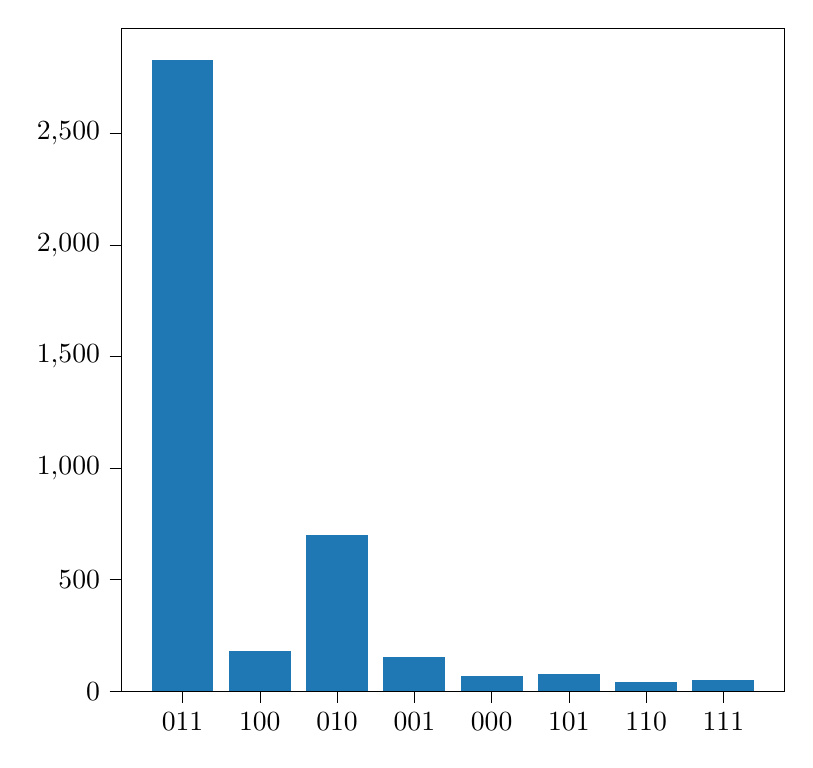
\begin{tikzpicture}

\definecolor{darkgray176}{RGB}{176,176,176}
\definecolor{steelblue31119180}{RGB}{31,119,180}

\begin{axis}[
height=10cm,
tick align=outside,
tick pos=left,
width=10cm,
x grid style={darkgray176},
xmin=-0.79, xmax=7.79,
xtick style={color=black},
xtick={0,1,2,3,4,5,6,7},
xticklabels={011,100,010,001,000,101,110,111},
y grid style={darkgray176},
ymin=0, ymax=2971.5,
ytick style={color=black}
]
\draw[draw=none,fill=steelblue31119180] (axis cs:-0.4,0) rectangle (axis cs:0.4,2830);
\draw[draw=none,fill=steelblue31119180] (axis cs:0.6,0) rectangle (axis cs:1.4,179);
\draw[draw=none,fill=steelblue31119180] (axis cs:1.6,0) rectangle (axis cs:2.4,700);
\draw[draw=none,fill=steelblue31119180] (axis cs:2.6,0) rectangle (axis cs:3.4,151);
\draw[draw=none,fill=steelblue31119180] (axis cs:3.6,0) rectangle (axis cs:4.4,69);
\draw[draw=none,fill=steelblue31119180] (axis cs:4.6,0) rectangle (axis cs:5.4,78);
\draw[draw=none,fill=steelblue31119180] (axis cs:5.6,0) rectangle (axis cs:6.4,39);
\draw[draw=none,fill=steelblue31119180] (axis cs:6.6,0) rectangle (axis cs:7.4,50);
\end{axis}

\end{tikzpicture}
